\chapter{High Low Guessing Game}
\label{chapter:RPS}
\graphicspath{ {./Lab04HighLow/Fig} }

\section{Outcomes and Objectives}

The outcome of this lab is to instantiate a guessing game using 
common logic building blocks.
on the FPGA development board. 
Through this process you will achieve the following
learning objectives.
\begin{itemize}
	\item \Paste{bok:REP_WordStatement}
	\item \Paste{bok:REP_TruthTable}
\end{itemize}

\section{The Guessing Game}

The guessing game is a two-person game where, one player is the guesser
and the other, an honest, secret keeper. The game starts with the secret
keeper generating a \emph{secret number} between {[}\textbf{0} and
\textbf{15}{]}, inclusive. Once the \emph{secret number} is decided, the
guesser makes a \emph{guess}, a number in the interval {[}\textbf{0} to
\textbf{15}{]} inclusive, and tells this to the secret keeper. The
secret keep then replies to the guesser if \emph{guess} is less than,
equal to, or greater than the \emph{secret number}. The game continues
with repeated guesser/secret keeper exchanges until the guesser
correctly identifies the \emph{secret number}.

\begin{figure}[ht]
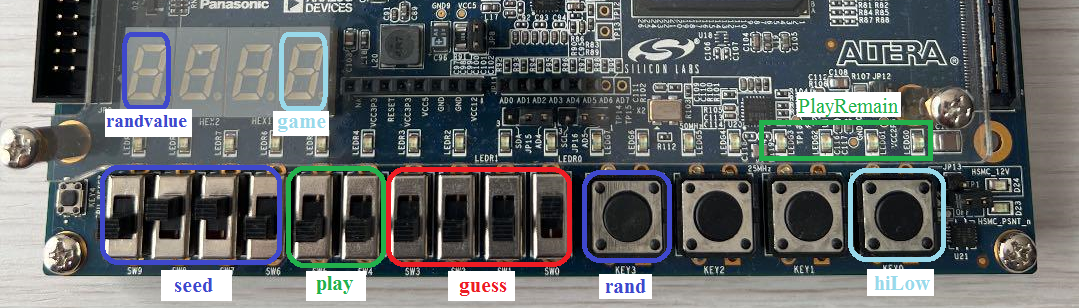
\includegraphics{image1.png}
\caption{The input and output you should use to realize the High/Low Guessing game.}
\label{fig:inputOutputDevBoard}
\end{figure}

Your goal in this lab is to create a digital version of the guessing
game using the development board using the inputs and outputs shown in
Figure~\ref{fig:inputOutputDevBoard}. In this case, the FPGA will play the role of secret keeper.
You will enter a seed value using the \textbf{seed} slide switches. The
seed value will be ``randomized'' into a 4-bit \emph{secret number}
using a linear feedback shift generator (more about this later).
Pressing the \textbf{rand} button reveals the \textbf{4}-bit
\emph{secret number} as a \textbf{1} --digit hexadecimal value on the
\textbf{randValue} 7-segment displays. Obviously, the guesser should not
press the \textbf{rand} button during regular game play.

The player will make their guess about the secret number on the
\textbf{guess} slide switches. This \emph{guess} is compared to the
\emph{secret number} and the outcome is displayed on the \textbf{game}
7-segment display when the \textbf{hiLow} button is pressed. The
\textbf{game} 7-segment display will show:

\begin{itemize}
\item   `H' when \emph{guess} \textgreater{} \emph{secret number}
\item   `I' when \emph{guess} = \emph{secret number}
\item   `L' when \emph{guess} \textless{} \emph{secret number}
\end{itemize}

A player is only allowed \textbf{4} guesses to get the secret number. To
keep track of this, every time that the player makes a guess, they
increment the binary number on the \textbf{play} slide switches. When a
slide switch is in the up position, the bit value is 1 and when in the
down position, the bit value is 0. This means that the player needs to
understand how to count in binary. In order to make keeping track of the
number of guesses remaining, the number of illuminated green
\textbf{playRemaining} LEDs will equal the number of guesses left. For
example, if the binary value set on the \textbf{play} slide switches
equals \textbf{2}, then the right-most \textbf{2} green LEDs would be
illuminated. You should illuminate LEDs starting from the right side and
increasing towards the left side.

\section{System Architecture}
Use the system architecture shown in Figure~\ref{fig:guessGameSysArch} as your
guide to this design. Please note that lines with the same name in different places 
are connected together. For example, the signal \emph{randBut} connects the button input to the 
2:1 mux in the upper left corner of  the FPGA.

\begin{figure}[ht]
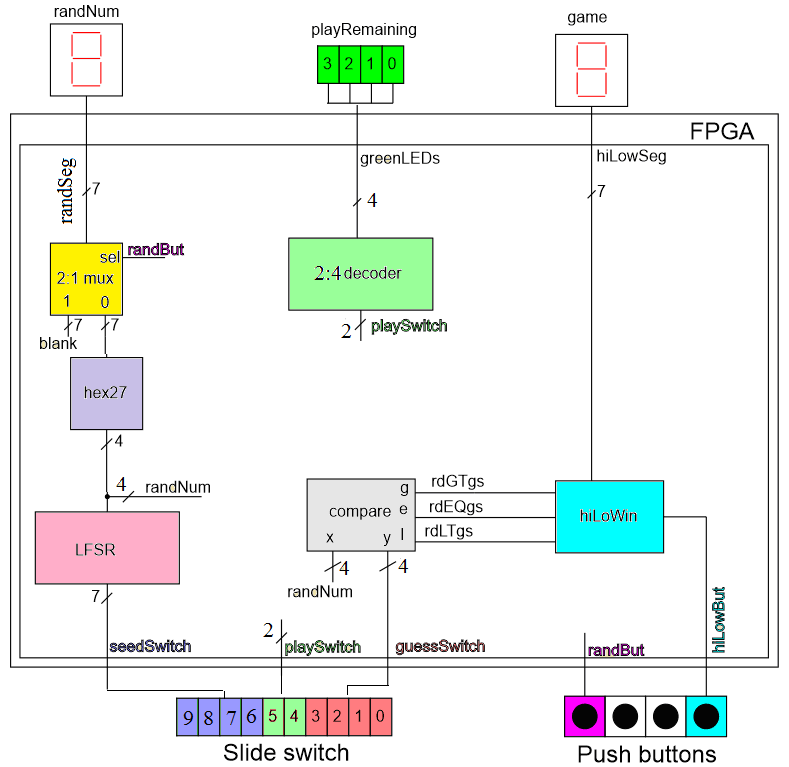
\includegraphics[width=0.6\paperwidth]{image2.png}
\caption{System architecture for the guessing game.}
\label{fig:guessGameSysArch}
\end{figure}

\section{Module: 2:1 Mux}

A 2:1 multiplexer, a mux for short, is a basic building block in many
digital systems. The 2:1 mux shown in Figure~\ref{fig:2x1MuxSymbol} routes one of the two
N-bit data inputs, \textbf{y\textsubscript{0}} or
\textbf{y\textsubscript{1}} to the N-bit output, \textbf{F}, depending
on the value of a 1-bit select signal, \textbf{s}. When \textbf{s} = 0,
\textbf{F}= \textbf{y\textsubscript{0}} and when \textbf{s} = 1,
\textbf{F}= \textbf{y\textsubscript{1}}. In other word, \textbf{F}
equals the \textbf{y} input whose subscript equals \textbf{s}.

\begin{figure}[ht]
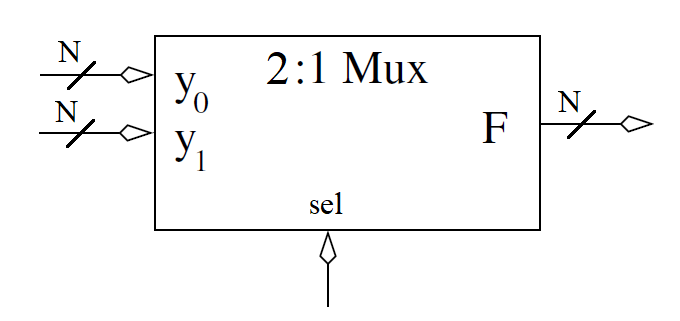
\includegraphics[width=0.4\paperwidth]{image3.png}
\caption{The schematic representation of a 2:1 mux.}
\label{fig:2x1MuxSymbol}
\end{figure}

You may notice that the data inputs of the 2:1 muxes in Figure~\ref{fig:guessGameSysArch}
 have
their \textbf{y\textsubscript{0}} and \textbf{y\textsubscript{1}} data
inputs denoted as `0' and `1' respectively. This is done to save space
and increase clarity in the schematic.

The Verilog code for a 2:1 mux is provided to you on Canvas. When
creating instances of the 2:1 mux, you will need to correctly order the
signals in the module instantiation. To do this, follow the
order shown in the module declaration shown in the top two lines in
Listing~\ref{listing:2x1muxVerilog}.

\begin{lstlisting}[language=Verilog,
 caption={Top, module definition for a 2:1 mux.  Bottom, module instantation 
 of a 2:1 mux in Figure~\ref{fig:guessGameSysArch}.},
 label={listing:2x1muxVerilog},
 frame=single]
// Module definition for the 2:1 mux
module genericMux2x1(y1, y0, sel, f);

// Module instantation for a 2:1 mux in the hiLow digital circuit
genericMux2x1 #(7) muxHex(7'b1111111, RandHex, randBut, randSeg);
\end{lstlisting}

The signal width, \textbf{N}, shown in Figure~\ref{fig:2x1MuxSymbol} is a placeholder for
an integer value that describes the width of the \emph{y1, y0, F} signals.  You can
specify this width when you instantiate a \emph{genericMux2x1} module using the \#()
specifier immediately after \emph{genericMux2x1} as shown in the bottom line of code in Listing 1. 

A component
that you can instantiate with different signal widths is called
``generic'' and often used in the module's name.  Often generics
have a default value, for the genericMux2x1 it is 8-bit. This is 
worth mentioning because if you forget to include \#(7) in your
instantation, the compiler will generate a warning that is easy to
overlook and your design will not simulate or synthesize correctly.
If you suspect this is occuring in your design,  look in the Compilation
Report tab -\textgreater{} Analysis \& Synthesis folder -\textgreater{}
Connectivity Checks folder. Click on the offending module and you will
see the following error report. 

\begin{figure}[ht]
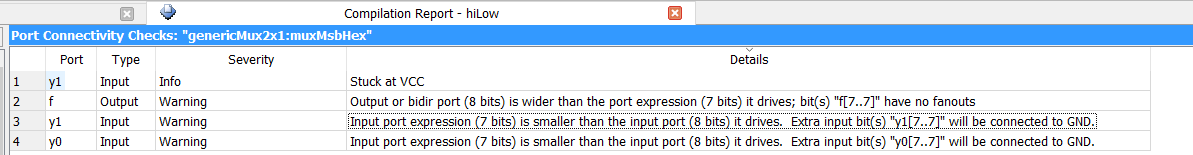
\includegraphics{image4.png}
\caption{Forgetting the generic specifier in a 2:1 Mux will generate this report.}
\label{fig:vectorSizeWarnings}
\end{figure}

\hypertarget{compare-module}{%
\section{Module: Compare}\label{compare-module}}

A N-bit comparator is a basic building block in many digital systems.
The N-bit comparator shown in Figure~\ref{fig:comparatorSymbol} 
checks the relative magnitude of
the two N-bit inputs \textbf{x} and \textbf{y} and sets one of the three
outputs equal to 1, one's-hot output, depending on their relation to
each other.

\begin{figure}[ht]
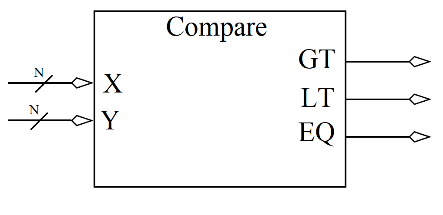
\includegraphics[width=0.4\paperwidth]{image5.png}
\caption{A schematic representation of a N-bit comparator.}
\label{fig:comparatorSymbol}
\end{figure}

The relationship between the inputs and outputs is given in the
following list. Note that the order of the inputs is important as
\textbf{X} is always on the left side of the relational operator.

\begin{itemize}
\item    \textbf{GT} = 1 when \textbf{X} \textgreater{} \textbf{Y} else  \textbf{GT} = 0
\item    \textbf{EQ} = 1 when \textbf{X} == \textbf{Y} else \textbf{EQ} = 0
\item    \textbf{LT} = 1 when \textbf{X} \textless{} \textbf{Y} else   \textbf{LT} = 0
\end{itemize}

The Verilog code for the N-bit comparator is available on Canvas.
When creating instances of the comparator, you will need to correctly
order the signals in the module instantiation. To do this, follow the
order shown in the module definition shown in the top two lines in
Listing ~ref{listing:comparatorVerilog}.

\begin{lstlisting}[language=Verilog,
 caption={Top, the module definition for the comparator.  Bottom, module
 instantiation of a comparator in Figure~\ref{fig:comparatorSymbol}. Remove the 
component instantiation line break in your code.},
 label={listing:comparatorVerilog},
 frame=single]
// Module definition for the comparator
module genericComparator(x, y, gt, eq, lt);

// Module instantiation for a compataror in the hiLow digital circuit
genericComparator #(4) randVsGuess(randNum, guessSwitch, \
		 randGTguess, randEQguess, randLTguess);
\end{lstlisting}

Like the mux, the comparator is a generic module. This means that you
need to specify the width of the \textbf{X} and \textbf{Y} vectors 
using the \#() specifier. The same warnings about vector size mismatch 
applies to comparators.


\section{Module: hexToSevenSeg}
You should use the hexToSevenSeg module you developed in a
previous lab. Note, the name of this module was shortened in Figure~\ref{fig:guessGameSysArch}
to hex27 in order to save space and make the schematic more
readable.


\section{Module: 2:4 Decoder}


The module labeled 2:4 decoder interprets the 2-bit input
s\textsubscript{1}, s\textsubscript{0} as a 2-bit binary number that we
will call \textbf{s}. All the y outputs whose subscript is less than or
equal to \textbf{s} will have an output of 1. All the y outputs whose
subscript is greater than \textbf{s} will have an output of 0.

\begin{figure}[ht]
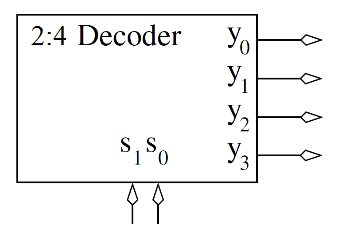
\includegraphics[width=0.3\paperwidth]{image6.png}
\caption{A 2:4 decoder.}
\label{fig:2x4decoderSymbol}
\end{figure}

The first few rows for the truth table for the 2:4 decoder are shown in
Table~\ref{table:decoderTruthTable}.

\begin{longtable}[]{@{}
 | >{\raggedright\arraybackslash}p{(\columnwidth - 10\tabcolsep) * \real{0.1688}} |
  >{\raggedright\arraybackslash}p{(\columnwidth - 10\tabcolsep) * \real{0.1688}} |
  >{\raggedright\arraybackslash}p{(\columnwidth - 10\tabcolsep) * \real{0.1696}} |
  >{\raggedright\arraybackslash}p{(\columnwidth - 10\tabcolsep) * \real{0.1696}} |
  >{\raggedright\arraybackslash}p{(\columnwidth - 10\tabcolsep) * \real{0.1617}} |
  >{\raggedright\arraybackslash}p{(\columnwidth - 10\tabcolsep) * \real{0.1617}}|@{}}
\caption{Partial truth table for the 2:4 decoder.}
\label{table:decoderTruthTable}
\tabularnewline
\toprule()
\begin{minipage}[b]{\linewidth}\raggedright
s\textsubscript{1}
\end{minipage} & \begin{minipage}[b]{\linewidth}\raggedright
s\textsubscript{0}
\end{minipage} & \begin{minipage}[b]{\linewidth}\raggedright
y\textsubscript{3}
\end{minipage} & \begin{minipage}[b]{\linewidth}\raggedright
y\textsubscript{2}
\end{minipage} & \begin{minipage}[b]{\linewidth}\raggedright
y\textsubscript{1}
\end{minipage} & \begin{minipage}[b]{\linewidth}\raggedright
y\textsubscript{0}
\end{minipage} \\
\midrule()
\endfirsthead
\toprule()
\begin{minipage}[b]{\linewidth}\raggedright
s\textsubscript{1}
\end{minipage} & \begin{minipage}[b]{\linewidth}\raggedright
s\textsubscript{0}
\end{minipage} & \begin{minipage}[b]{\linewidth}\raggedright
y\textsubscript{3}
\end{minipage} & \begin{minipage}[b]{\linewidth}\raggedright
y\textsubscript{2}
\end{minipage} & \begin{minipage}[b]{\linewidth}\raggedright
y\textsubscript{1}
\end{minipage} & \begin{minipage}[b]{\linewidth}\raggedright
y\textsubscript{0}
\end{minipage} \\
\midrule()
\endhead
0 & 0 & 1 & 1 & 1 & 1 \\ \hline
0 & 1 & 0 & 1 & 1 & 1 \\ \hline
1 & 0 & 0 & 0 & 1 & 1 \\
\bottomrule()
\end{longtable}

While this implementation may look odd, it converts the user's selection
on the \textbf{play} slide-switches to show the correct number of plays
remaining for the user on the LEDs.

You should implement the 2:4 decoder in the hiLow module using an
always/case statement similar to the one used to implement your
hexToSevenSeg. You should put this Verilog code in the hiLow module as a
(large) concurrent statement. \textbf{This means that you should not
have a separate Verilog file for the 2:4 decoder.} Remember that the
output type from an always/case statement must have the ``reg''
qualifier, not ``wire''.


\section{Module: hiLowWin}

The hiLowWin functionality converts the output from the comparator into
the illuminated patterns shown in Figure~\ref{fig:hiLowWinDisplay} 
when the \textbf{hiLow}
button is pressed. The ``I'' from ``wIn'' is needed because you cannot
make a ``W'' on a 7-segment display.

\begin{figure}[ht]
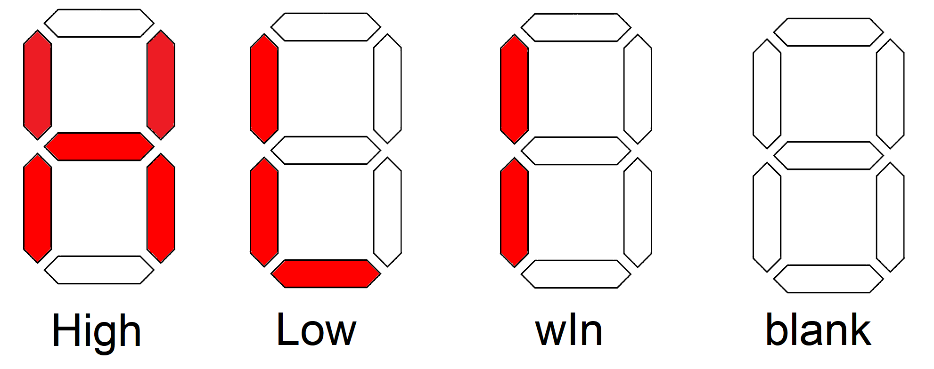
\includegraphics[width=0.5\paperwidth]{image7.png}
\caption{The illuminated patterns to inform the guesser about the
magnitude of their guess.}
\label{fig:hiLowWinDisplay}
\end{figure}

You should implement hiLowWin inside the hiLow module using an
always/case statement similar to the one used to implement your
hexToSevenSeg. You will need to create a vector out of the 4-separate
inputs using the parenthesis operator as shown in Listing~\ref{listing:hiLowWinVerilog}. 
Note that the code shown Listing~\ref{listing:hiLowWinVerilog} is incomplete.

\begin{lstlisting}[language=Verilog,
 caption={Starter code for the hiLowWin module.},
 label={listing:hiLowWinVerilog},
 frame=single]
 always @(*)
	case ({hotColdBut, hotWire, warmWire, coldWire})            
		4'b0001: hotColdSeg = 7'bxxxxxxx;				
		default: hotColdSeg = 7'bxxxxxxx;
	endcase  
 \end{lstlisting}

You should put this Verilog code in the hiLow module as one of the many
concurrent statement. This means that you \uline{should not} have a
separate Verilog file for the hiLowWin. Remember that the output type
from an always/case statement must have the ``reg'' qualifier, not
``wire''.


\section{Module: LFSR}

A linear feedback shift register (LFSR) is a digital circuit that
generates a pseudo-random sequence of numbers starting from a seed
value. Since we do not yet have storage devices in our class, we will
implement a LFSR that performs a single iteration of the randomization
step as shown in Figure~\ref{fig:lfsrOperation}.

\begin{figure}[ht]
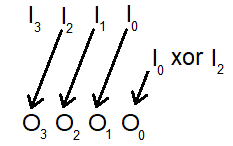
\includegraphics{image8.png}
\caption{A) A schematic illustration of a 4-bit LFSR operation. B) The
input 4b'1110 produced the output 4b'1101.}
\label{fig:lfsrOperation}
\end{figure}

Figure~\ref{fig:lfsrOperation} shows the input bits I\textsubscript{2} \ldots{}
I\textsubscript{0} being shifted one bit to the left on their way to the
outputs O\textsubscript{3} \ldots{} O\textsubscript{1}. The output
O\textsubscript{0} is formed by computing I\textsubscript{2} \^{}
I\textsubscript{0} where ``\^{}'' is the xor operation.

Let's use Table~\ref{table:lfsrOperations} to 
understand what happens if the input in 
Figure~\ref{fig:lfsrOperation}
was 7'b1110, which, when interpreted as a decimal number, is 14. The upper
3-bits of output are formed by shifting the input left by one bit. The
least significant bit of the output is formed by computing 1 \^{} 0
which equals 1. The resulting output is 4'b1101, when interpreted as a
decimal number, equals 13. Fill in the next blank row of Table 2 using
decimal 13 as an input. Repeat for the last row of the table.

\begin{longtable}[]{@{}
 | >{\raggedright\arraybackslash}p{(\columnwidth - 8\tabcolsep) * \real{0.1999}} |
  >{\raggedright\arraybackslash}p{(\columnwidth - 8\tabcolsep) * \real{0.1999}} |
  >{\raggedright\arraybackslash}p{(\columnwidth - 8\tabcolsep) * \real{0.2001}} |
  >{\raggedright\arraybackslash}p{(\columnwidth - 8\tabcolsep) * \real{0.2001}} |
  >{\raggedright\arraybackslash}p{(\columnwidth - 8\tabcolsep) * \real{0.2001}}|@{}}
\caption{The first iteration of the LFSR shown in Figure~\ref{fig:lfsrOperation} 
when started at decimal 14.}
\label{table:lfsrOperations}
\tabularnewline
\toprule()
\begin{minipage}[b]{\linewidth}\raggedright
O\textsubscript{3}
\end{minipage} & \begin{minipage}[b]{\linewidth}\raggedright
O\textsubscript{2}
\end{minipage} & \begin{minipage}[b]{\linewidth}\raggedright
O\textsubscript{1}
\end{minipage} & \begin{minipage}[b]{\linewidth}\raggedright
O\textsubscript{0}
\end{minipage} & \begin{minipage}[b]{\linewidth}\raggedright
decimal
\end{minipage} \\
\midrule()
\endfirsthead
\toprule()
\begin{minipage}[b]{\linewidth}\raggedright
O\textsubscript{3}
\end{minipage} & \begin{minipage}[b]{\linewidth}\raggedright
O\textsubscript{2}
\end{minipage} & \begin{minipage}[b]{\linewidth}\raggedright
O\textsubscript{1}
\end{minipage} & \begin{minipage}[b]{\linewidth}\raggedright
O\textsubscript{0}
\end{minipage} & \begin{minipage}[b]{\linewidth}\raggedright
decimal
\end{minipage} \\
\midrule()
\endhead
1 & 1 & 1 & 0 & 14 \\ \hline
1 & 1 & 0 & 1 & 13 \\ \hline
& & & & \\ \hline
& & & & \\
\bottomrule()
\end{longtable}

If you continued the output from the shift operation performed in Table~\ref{table:lfsrOperations} 
you would eventually find a decimal number that repeats because there
are only 16 different combinations of 4-bits. Call this repeat number
the nexus. The length of the sequence of numbers a nexus back to itself
is the length of the sequence. The length of the sequence generated by
the operation in Figure~\ref{fig:lfsrOperation} is 15. This means that if Table 2 had 15 rows
and you filled them all in, you would get 14 on the
14\textsuperscript{th} row. Can you figure out what number is excluded
from the sequence?

For the lfsr module, you need to:

\begin{itemize}
\item
  Use the module declaration:\\
\verb+ module lfsr(Seed, outputRand);+

\item
  Make the input and outputs vectors with wire type.
\item
  \protect\hypertarget{lfsr_verilog}{}{}Use 4 assign statements to give
  each bit of output a value.
\item
  \protect\hypertarget{lfsr_testbench}{}{}Complete the testbench for the
  lfsr module. Create timing diagram that asserts the four inputs listed
  in Table~\ref{table:lfsrOperations} 
  waiting \#20 between inputs. Zoom to fill the available
  horizontal space with the waveform. Color inputs green and outputs
  red. Switch radix to unsigned decimal for input and output (right
  click on signal name in wave pane and select radix -\textgreater{}
  unsigned).
\end{itemize}

\section{Module: hiLow}

The hiLow module stitches together all the modules and contains all 
the signals shown in
Figure~\ref{fig:guessGameSysArch}. The module declaration is provided 
below to assist your pin assignment.

\begin{verbatim}
module hiLow(seedSwitch, playSwitch, guessSwitch, randBut, hiLowBut,
			randSeg, greenLEDs, hiLowSeg);
\end{verbatim}

To complete this module, you will need to instantiate all the modules in
Figure~\ref{fig:guessGameSysArch}. To provide guidance on this process
let's focus on the 2:1 mux from Figure~\ref{fig:snippetFromSysArch}.  This
2:1 mux is repsoduced in Figure~\ref{fig:snippetFromSysArch}.

\begin{figure}[ht]
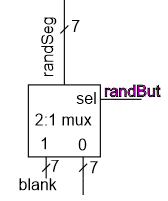
\includegraphics{image9.png}
\caption{A small piece of hardware from Figure~\ref{fig:guessGameSysArch}.}
\label{fig:snippetFromSysArch}
\end{figure}


Let's write the Verilog code to instantiate the 2:1 mux.
The first step that you need to take is to give EVERY signal in the
system architecture a name or constant value. With respect to Figure~\ref{fig:snippetFromSysArch},
the output of the 2:1 mux is already named \textbf{randSeg} and the
select line is named \textbf{randBut}. The data input y1 will have a
constant value \textbf{7b'1111111}, needed to produce a blank 7-segment
display. The input y0 is the output from a hexToSevenSeg module, a signal 
named \textbf{RandHex}.

The second step is to know the order of the parameters in the 2:1 mux
module declaration. This was given earlier as:

\verb+ module genericMux2x1(y1, y0, sel, f); +


The third step is instantiating the 2:1 mux in Verilog. To do this:

\begin{itemize}
\item
  Define the width of the data input and data output of the mux
  (7-bits),
\item
  Give the 2:1 mux instance a descriptive and unique name. 
  For example, \textbf{muxHex},
\item
  Put the system architecture signals in their corresponding locations
  in the module

\verb+ genericMux2x1 #(7) muxHex(7\textquotesingle b1111111, RandHex, randBut, randSeg); +
\end{itemize}

Once you get the hang of it, you are just translating the system
architecture of Figure~\ref{fig:guessGameSysArch} into words.

For the hiLow module, you should:

\begin{itemize}
\item
  Use the module declaration:

\begin{verbatim}
module hiLow(seedSwitch, playSwitch, guessSwitch, randBut, hiLowBut,
		randSeg, greenLEDs, hiLowSeg); 
\end{verbatim}

\item
  Make the \verb+seedSwitch, playSwitch, seedSwitch+ inputs vectors with the
  left switch the MSB. You will need to keep this consistent with the
  pin assignment that you will compete next.
\item
  The \verb+randBut, hiLowBut+ inputs are not vectors.
\item
  Use a vector for the \verb+randSeg+ output with wire type.
\item
  Use a vector for the \verb+greenLEDs, hiLowSeg+ output with reg type.
\item
  My module had 3 internal vectors (wire type) and 3 internal one bit
  signals (shown in the system architecture).
\end{itemize}

\section{Testbench}

  Run the testbench for the hiLow module provided on Canvas. Produce a
  timing diagram with the following characteristics. Zoom to fill the
  available horizontal space with the waveform. Color inputs green and
  outputs red. Order the traces from top to bottom as shown in the 
  \hypertarget{hlgg:signalColor}{following table}.

\begin{tabular}{p{4cm}p{4cm}p{4cm}}
signal & radix & color trace \\ \hline
    t\_seedSwitch & unsigned  & green  \\
    t\_guessSwitch & unsigned & green  \\
    t\_playSwitch & unsigned & green  \\
    t\_randBut & default & green  \\
    t\_hiLowBut & default & green  \\
    LFSR output & unsigned & yellow \\
    t\_randSeg & hex & red  \\
    t\_hiLowSeg & hex & red  \\
    t\_greenLEDs & default & red  \\
  \end{tabular}



\section{Pin-Assignment and Synthesis}

Use the image of the development board in 
Figure~\ref{fig:inputOutputDevBoard} and the information
in the board User Guide to determine the FPGA pins associated with the
input and output devices used by the hiLow module. 

\begin{longtable}[]{@{}
|  >{\raggedright\arraybackslash}p{(\columnwidth - 4\tabcolsep) * \real{0.3396}}|
  >{\raggedright\arraybackslash}p{(\columnwidth - 4\tabcolsep) * \real{0.3718}}|
  >{\raggedright\arraybackslash}p{(\columnwidth - 4\tabcolsep) * \real{0.2886}}|@{}}
\toprule()
\caption{Pin-Assignment for the High Low Guessing Game.}
\label{table:hlggPinAssignment} \tabularnewline
Segment & randSeg & hiLowSeg \\
\midrule()
\endhead
seg{[}6{]} & PIN\_AC22 & PIN\_Y18 \\ \hline
seg{[}5{]} & & \\ \hline
seg{[}4{]} & & \\ \hline
seg{[}3{]} & & \\ \hline
seg{[}2{]} & & \\ \hline
seg{[}1{]} & & \\ \hline
seg{[}0{]} & & \\
\bottomrule()
\end{longtable}

\begin{longtable}[]{@{}
|  >{\raggedright\arraybackslash}p{(\columnwidth - 6\tabcolsep) * \real{0.2596}} |
  >{\raggedright\arraybackslash}p{(\columnwidth - 6\tabcolsep) * \real{0.2505}} |
  >{\raggedright\arraybackslash}p{(\columnwidth - 6\tabcolsep) * \real{0.2542}} |
  >{\raggedright\arraybackslash}p{(\columnwidth - 6\tabcolsep) * \real{0.2357}}|@{}}
\toprule()
 & seedSwitch & playSwitch & guessSwitch \\ 
\midrule()
\endhead
slide{[}3{]} & PIN\_AE19 & N/A & \\  \hline
slide{[}2{]} & & N/A & \\ \hline
slide{[}1{]} & & & \\ \hline
slide{[}0{]} & & & \\
\bottomrule()
\end{longtable}

\begin{longtable}[]{@{}
|  >{\raggedright\arraybackslash}p{(\columnwidth - 4\tabcolsep) * \real{0.3334}} |
  >{\raggedright\arraybackslash}p{(\columnwidth - 4\tabcolsep) * \real{0.3334}} |
  >{\raggedright\arraybackslash}p{(\columnwidth - 4\tabcolsep) * \real{0.3333}}|@{}}
\toprule()

randBut & Key{[}3{]} & \\
\midrule()
\endhead
\begin{minipage}[t]{\linewidth}\raggedright
hiLowBut
\end{minipage} & Key{[}0{]} & \\
\bottomrule()
\end{longtable}

\begin{longtable}[]{@{}
|  >{\raggedright\arraybackslash}p{(\columnwidth - 6\tabcolsep) * \real{0.2499}} |
  >{\raggedright\arraybackslash}p{(\columnwidth - 6\tabcolsep) * \real{0.2499}} |
  >{\raggedright\arraybackslash}p{(\columnwidth - 6\tabcolsep) * \real{0.2501}} |
  >{\raggedright\arraybackslash}p{(\columnwidth - 6\tabcolsep) * \real{0.2501}}|@{}}
\toprule()
\begin{minipage}[b]{\linewidth}\raggedright
G{[}3{]}
\end{minipage} & \begin{minipage}[b]{\linewidth}\raggedright
G{[}2{]}
\end{minipage} & \begin{minipage}[b]{\linewidth}\raggedright
G{[}1{]}
\end{minipage} & \begin{minipage}[b]{\linewidth}\raggedright
G{[}0{]}
\end{minipage} \\
\midrule()
\endhead
& & & \\
\bottomrule()
\end{longtable}

Complete the pin-assignment in Quartus, compile your design and download to the
FGPA development boards.  If you are having difficulty getting your circuit to work
correctly, please refer to Section~\ref{section:guessGameDebugging} for some 
useful debugging tips. 

Once you get your design working, demonstrate it to a member of the 
lab team.  


\section{Turn in}

You may work in teams of at most two. Make a record of your response to
the items below and turn them in a single copy as your team's solution
on Canvas using the instructions posted there. Include the names of both
team members at the top of your solutions. Use complete English
sentences to introduce what each of the following listed items (below)
is and how it was derived. In addition to this submission, you will be
expected to demonstrate your circuit at the beginning of your lab
section next week.

\subsubsection{Module: LFSR }
\begin{itemize}
\item
  \protect\hyperlink{lfsr_verilog}{Link} Verilog code for the body of
  the module (courier 8-point font single spaced), leave out header
  comments.
\item A completed Table~\ref{table:lfsrOperations}.
\item
  \protect\hyperlink{lfsr_testbench}{Link} Complete the testbench for
  the lfsr module. Create timing diagram that asserts the four inputs
  listed in Table~\ref{table:lfsrOperations} waiting \#20 between inputs. Zoom to fill the
  available horizontal space with the waveform. Color inputs green and
  outputs red. Switch radix to unsigned decimal for input and output
  (right click on signal name in wave pane and select radix
  -\textgreater{} unsigned).
\end{itemize}

\subsubsection{Module: hiLow}


\begin{itemize}
\item
  Verilog code for the body of the hiLow module (courier 8-point
  font single spaced), leave out header comments.
\item
  Run the testbench for the hiLow module provided on Canvas.
  Produce a timing diagram according to
  \hyperlink{hlgg:signalColor}{this table}. Zoom to
  fill the available horizontal space with the waveform. 
\end{itemize}

\subsubsection{Pin-Assignment and synthesis}

\begin{itemize}
\item Completed pin assignment table for all the signals in the hiLow module in Table~\ref{table:hlggPinAssignment}.
\end{itemize}


\section{Debugging Tips}
\label{section:guessGameDebugging}
This laboratory typically generates a variety of new errors that you 
have not seen before.  This section on useful debugging techniques 
will help you more effectively 
interpert the compilers output to locate errors in your code.
The following is an example story of someone debugging their code...

After you put together all the components, you can run Start Analysis \&
Elaboration. It may take you a while to find all your errors.  Try
clicking on the Error icon (red x) or Warning icon (yellow
triangle) in the console area, to eliminate a lot of the clutter.

Th error below is a result of defining the output \verb+wire {[}7:0{]} greenLEDs+.
the output should have  \verb+reg{[}7:0{]} greenLEDs;+ because greenLEDs is the 
output of an always/case statement.

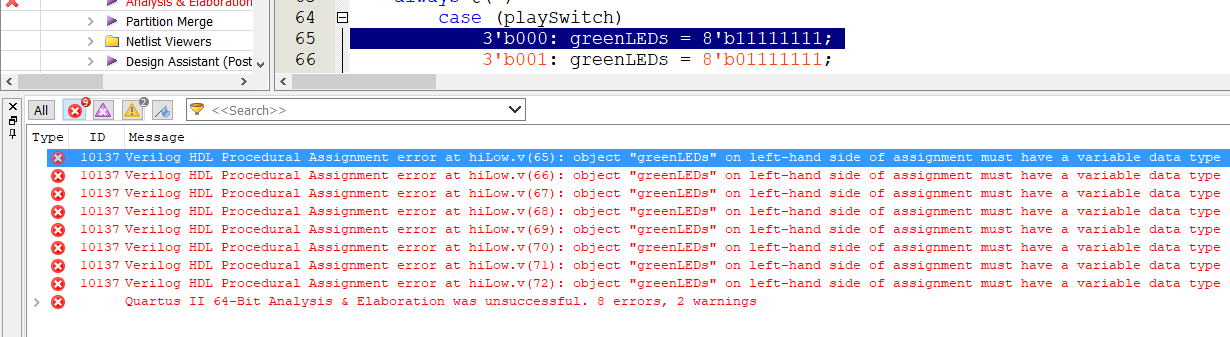
\includegraphics{image10.png}

The following error is the result of forgetting to include the declaration of randNum. 
The top warning always appears and the second is a result of an unused output on 
the adder (more about this in the next lab).

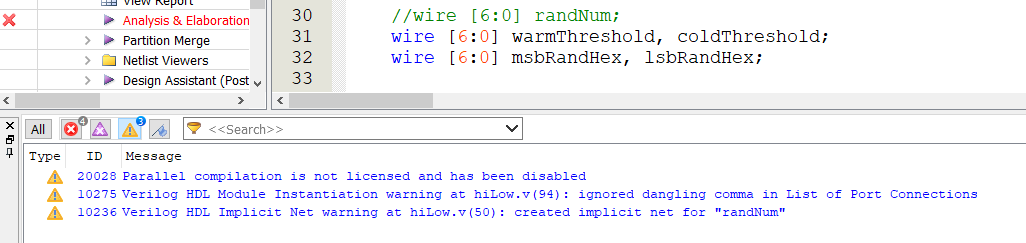
\includegraphics{image11.png}
Teh next error shows what happen when you accidentally leave a testbench as the 
top-level entity when attempting to synthesize.

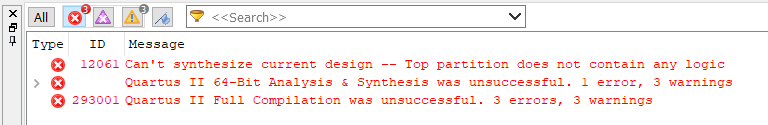
\includegraphics{image12.png}

These are all the Critical Warnings and Warnings that you will see on your final,
working version. You should NOT attempt to fix these ``errors''.

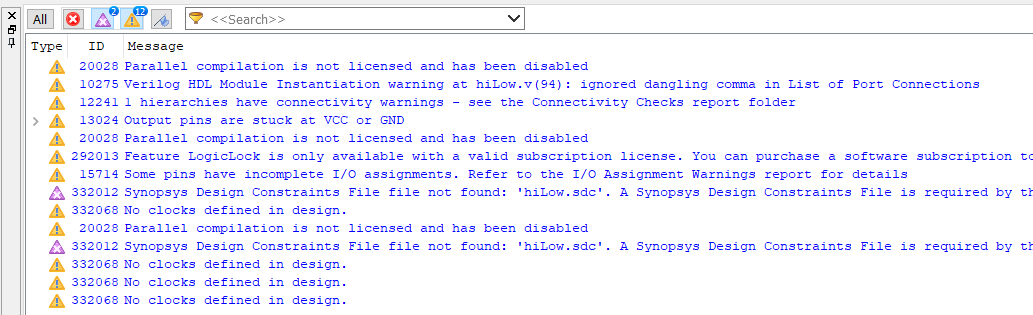
\includegraphics{image13.png}

The Connectivity Checks folder from the Compilation Report will help you
find weird connection problems that you may have inadvertently created
in your design. 
